\documentclass{article}

\usepackage{graphicx}
\usepackage{epstopdf}

\begin{document}

\section*{Stencil}

\begin{figure}[h!]
  \begin{center}
    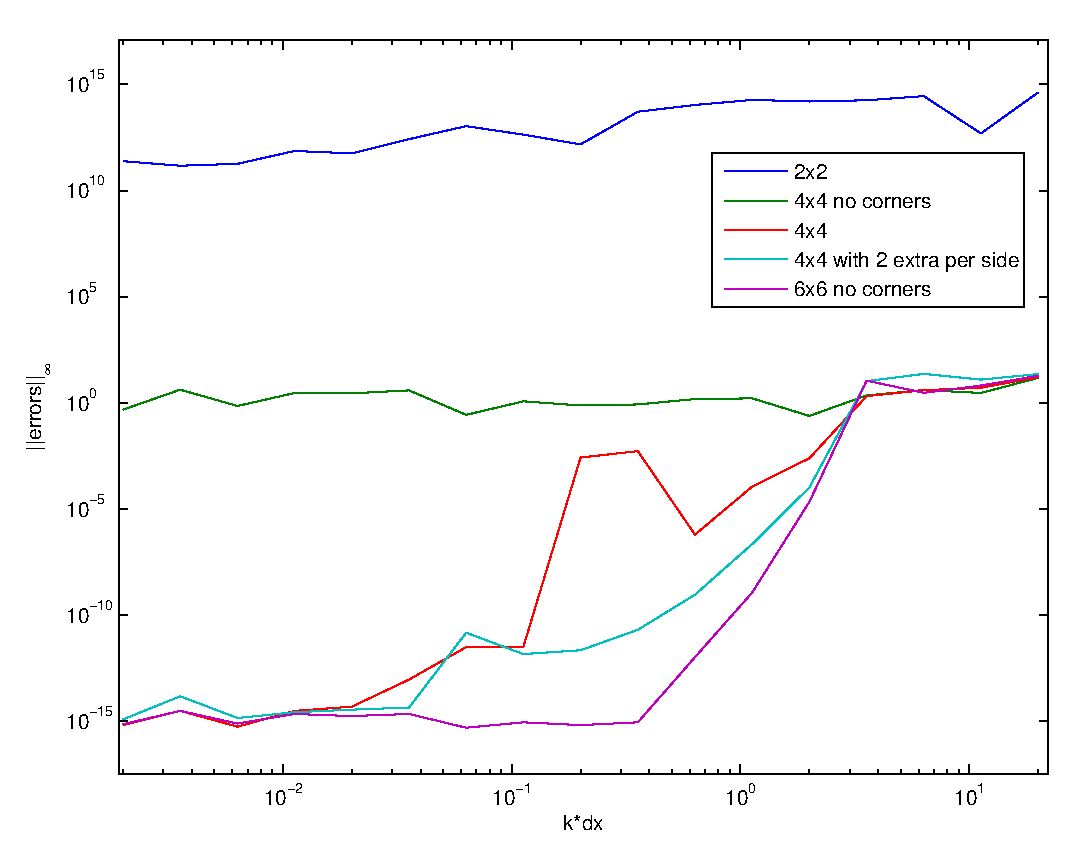
\includegraphics[width=0.75\textwidth]{figures/error_vs_kdx_over_stencils.eps}
    \caption{error norms in center square with M=12}
  \end{center}
\end{figure}

4x4 + 2/side seems like a good choice


\section*{$\rho$}
$\rho$ is upsampling ratio

Need to upsample enough to (almost) always resolve ambiguities. Very minor increased cost in evaluating Bessel's and matrix-vector multiplies.

I've been using $\rho=20$. Need to run tests with RPWs to see how often this fails.

\section*{$M$}

\begin{figure}[h!]
  \begin{center}
    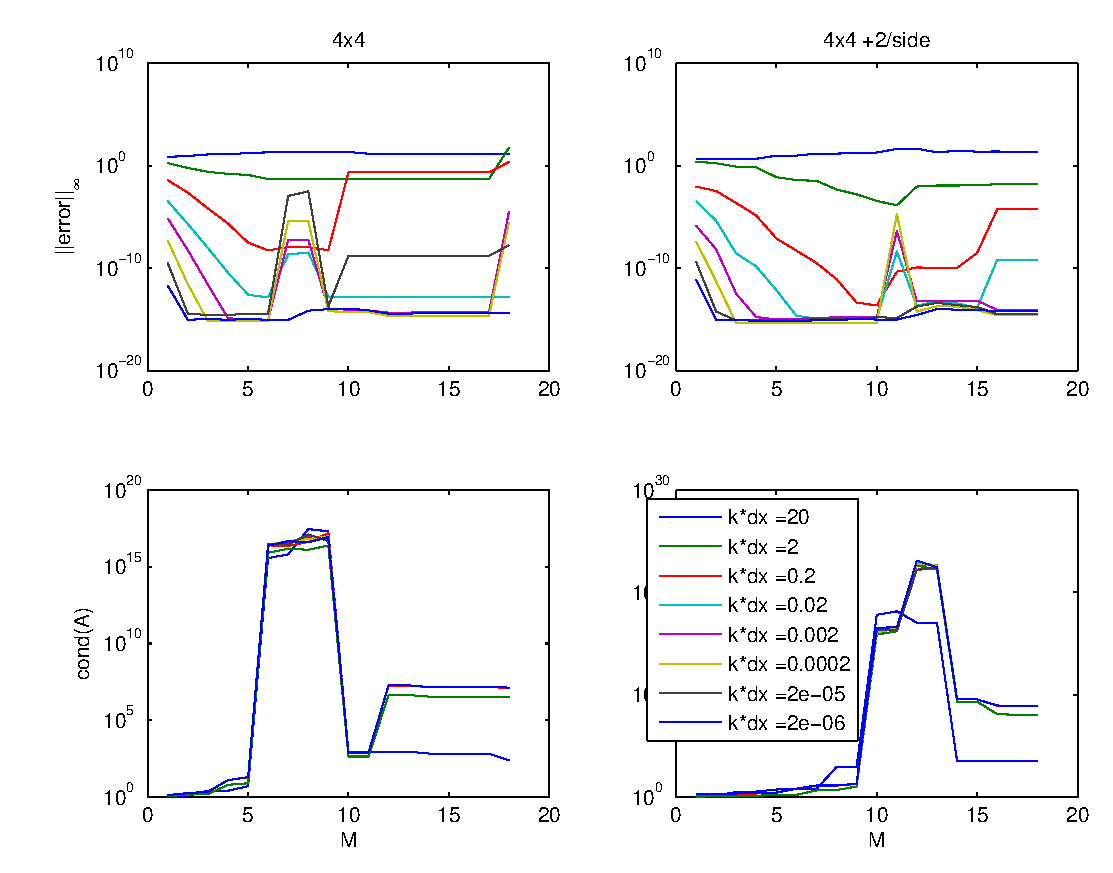
\includegraphics[width=0.75\textwidth]{figures/errors_and_conds_vs_M_over_kdx_4x4_and_4x4+2.eps}
    \caption{error norms and condition number for two stencil shapes}
    \label{fig:errors-and-conds}
  \end{center}
\end{figure}

See Fig. \ref{fig:errors-and-conds}.
Why is there a spike in error and condition number and why does it change with the stencil?

$M = 10$ should work well for 4x4 + 2/side

\section*{$\alpha$}
$\alpha := k \Delta x$

\begin{figure}[h!]
  \begin{center}
    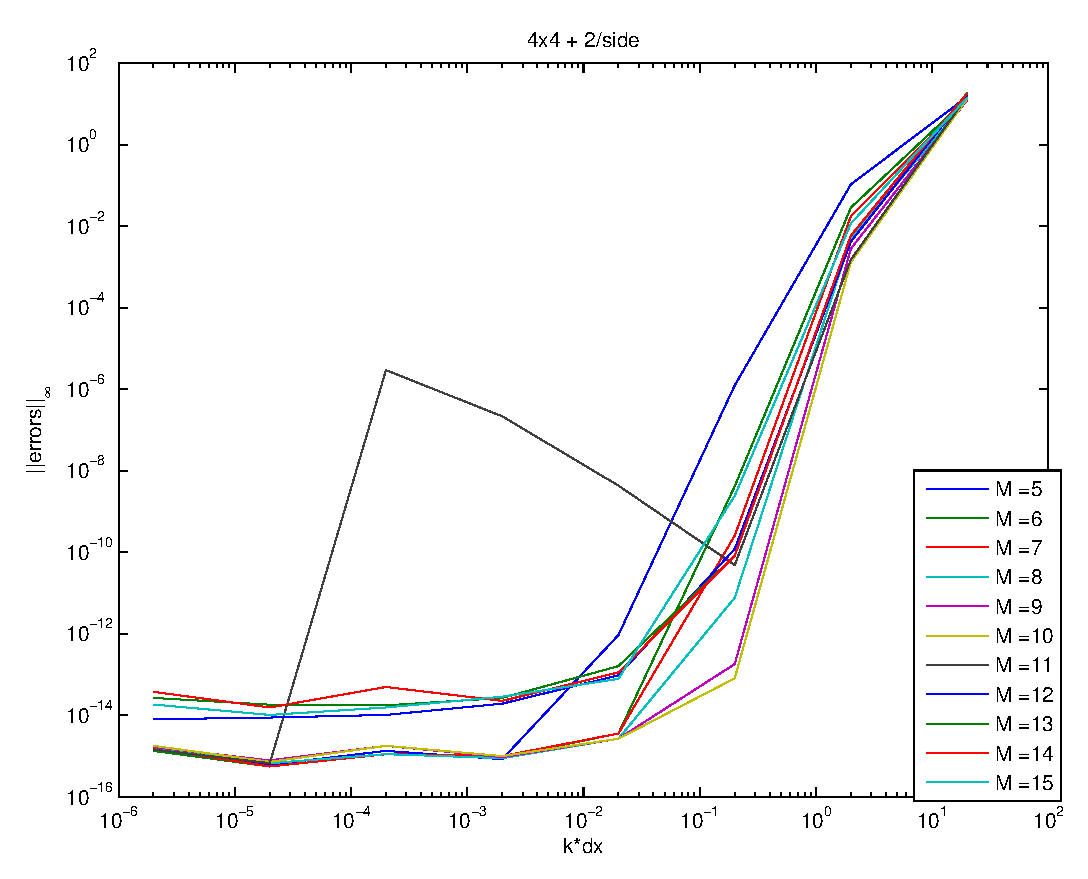
\includegraphics[width=0.75\textwidth]{figures/errors_vs_kdx_over_M_4x4+2.eps}
    \caption{error norms in center square of a 4x4 grid}
    \label{fig:errors}
  \end{center}
\end{figure}


See Fig. \ref{fig:errors}. We should aim for $\alpha < 10^{-1}$



\end{document}
